\documentclass[a4paper]{article}

%% Language and font encodings
\usepackage[english]{babel}
\usepackage[utf8x]{inputenc}
\usepackage[T1]{fontenc}

%% Sets page size and margins
\usepackage[a4paper,top=3cm,bottom=2cm,left=3cm,right=3cm,marginparwidth=1.75cm]{geometry}

%% Useful packages
\usepackage{amsmath}
\usepackage{graphicx}
\usepackage[colorinlistoftodos]{todonotes}
\usepackage[colorlinks=true, allcolors=blue]{hyperref}
\usepackage{float}


\title{Benchmarking P2C for HPC}
\author{Joseph Anthony C. Hermocilla}

\begin{document}
\maketitle

\begin{abstract}
We report some results of benchmarking P2C for HPC using NPB 3.3.1.
\end{abstract}

\section{Introduction}
In order to evaluate the performance of P2C for HPC, NPB Benchmark applications were tested. A 16-node cluster was deployed using vcluster.

\section{Results}

\subsection{Conjugate Gradient}

\begin{figure}[H]
\centering
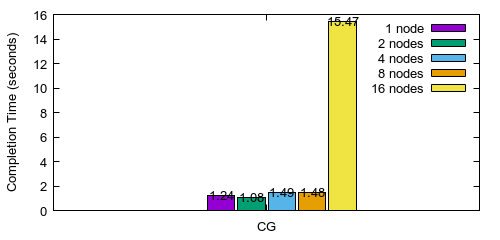
\includegraphics[width=0.8\textwidth]{figures/CGvA.png}
\caption{\label{fig:CGvA}This frog was uploaded via the project menu.}
\end{figure}

\begin{figure}[H]
\centering
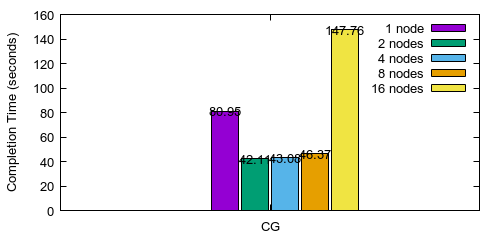
\includegraphics[width=0.8\textwidth]{figures/CGvB.png}
\caption{\label{fig:CGvB}This frog was uploaded via the project menu.}
\end{figure}

\subsection{Embarassingly Parallel}

\begin{figure}[H]
\centering
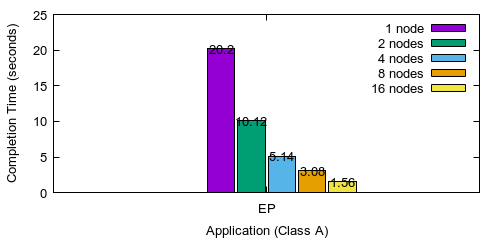
\includegraphics[width=0.8\textwidth]{figures/EPvA.png}
\caption{\label{fig:EPvA}This frog was uploaded via the project menu.}
\end{figure}

\begin{figure}[H]
\centering
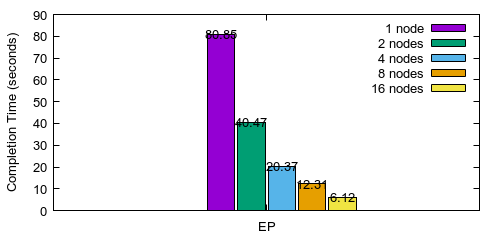
\includegraphics[width=0.8\textwidth]{figures/EPvB.png}
\caption{\label{fig:EPvB}This frog was uploaded via the project menu.}
\end{figure}


\subsection{Fourier Transform}

\begin{figure}[H]
\centering
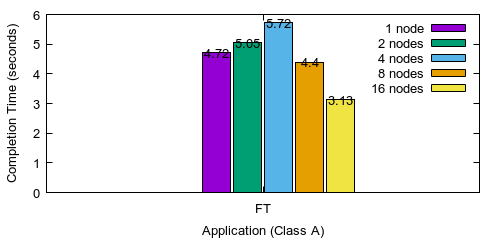
\includegraphics[width=0.8\textwidth]{figures/FTvA.png}
\caption{\label{fig:FTvA}This frog was uploaded via the project menu.}
\end{figure}

\begin{figure}[H]
\centering
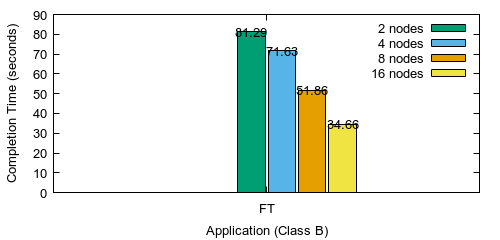
\includegraphics[width=0.8\textwidth]{figures/FTvB.png}
\caption{\label{fig:FTvB}This frog was uploaded via the project menu.}
\end{figure}

\subsection{Integer Sort}

\begin{figure}[H]
\centering
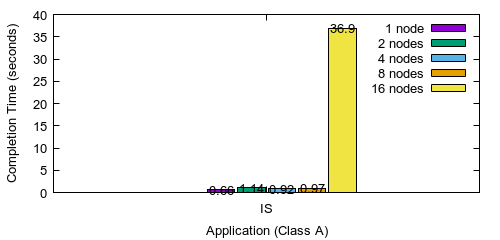
\includegraphics[width=0.8\textwidth]{figures/ISvA.png}
\caption{\label{fig:ISvA}This frog was uploaded via the project menu.}
\end{figure}

\begin{figure}[H]
\centering
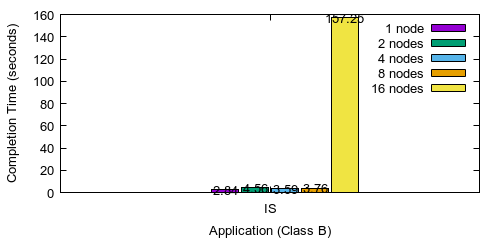
\includegraphics[width=0.8\textwidth]{figures/ISvB.png}
\caption{\label{fig:ISvB}This frog was uploaded via the project menu.}
\end{figure}

\subsection{Lower-Upper Gauss-Seidel Solver}

\begin{figure}[H]
\centering
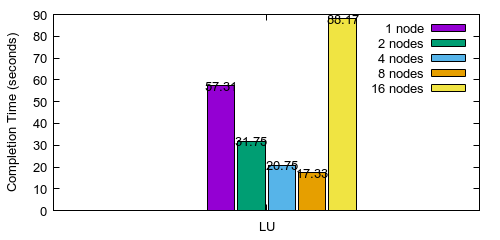
\includegraphics[width=0.8\textwidth]{figures/LUvA.png}
\caption{\label{fig:LUvA}This frog was uploaded via the project menu.}
\end{figure}

\begin{figure}[H]
\centering
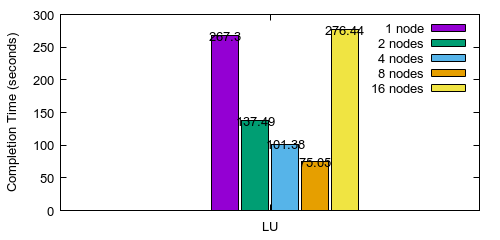
\includegraphics[width=0.8\textwidth]{figures/LUvB.png}
\caption{\label{fig:LUvB}This frog was uploaded via the project menu.}
\end{figure}

\subsection{Multi-Grid}

\begin{figure}[H]
\centering
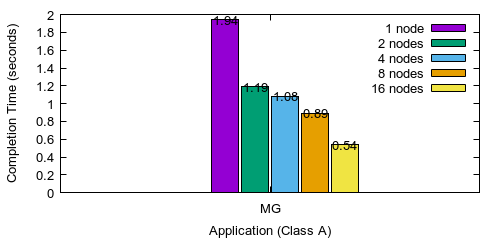
\includegraphics[width=0.8\textwidth]{figures/MGvA.png}
\caption{\label{fig:MGvA}This frog was uploaded via the project menu.}
\end{figure}

\begin{figure}[H]
\centering
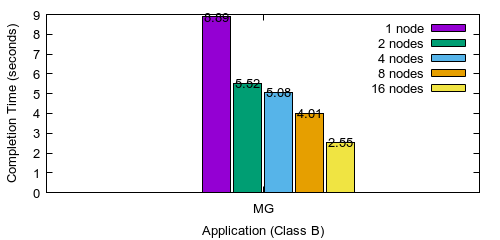
\includegraphics[width=0.8\textwidth]{figures/MGvB.png}
\caption{\label{fig:MGvB}This frog was uploaded via the project menu.}
\end{figure}

\bibliographystyle{alpha}
\bibliography{sample}

\end{document}